\chapter{Regression}

\section{Problem}
Since there is no obvious regression problem for our data set, we need to manufacture one ourselves. The way we have chosen to accomplish this is to make an attempt at predicting \emph{one} of the features from the all the \emph{other} features. This means that we extract one of the features from our feature set and make this our resulting \texttt{y} vector.

To keep it simple we will only look within a single class which in this report is the one for the digit 4 (chosen at random).

\section{Forward selection}
% Apply linear regression with forward selection and consider if transforming
% or combining attributes potentially may turn useful. For linear regression
% plotting the residual error vs. the attributes can give some insight into whether
% including a transformation of a variable can improve the model, i.e. potentially
% describe parts of the residuals.
Doing forward selection between all remaining 271 features will take a tremendous amount of time. Therefore we choose to only look within a certain part of the attributes (horizontal/vertical/radial histograms or in-out/out-in profiles), and limit it to these. \\

For our tests in this report we chose to stick to the in-out section of our features, which brings the feature count down to 72, which is manageable. From these we chose different features to try to predict and looked at the outcome, which usually either resulted in decent error rate or a quite bad error rate -- based on the feature we choose to predict.

Here is one example for each of these two cases:

\subsection*{Predicting feature 'In-out 50'}

We set the number 50 feature in the In-out section to be our feature to predict, and extract this from our feature set of the 72 features. 

Then we did forward feature selection with 10-fold cross-validation, and the selected features from this is shown below:

\begin{figure}[H]
\centering
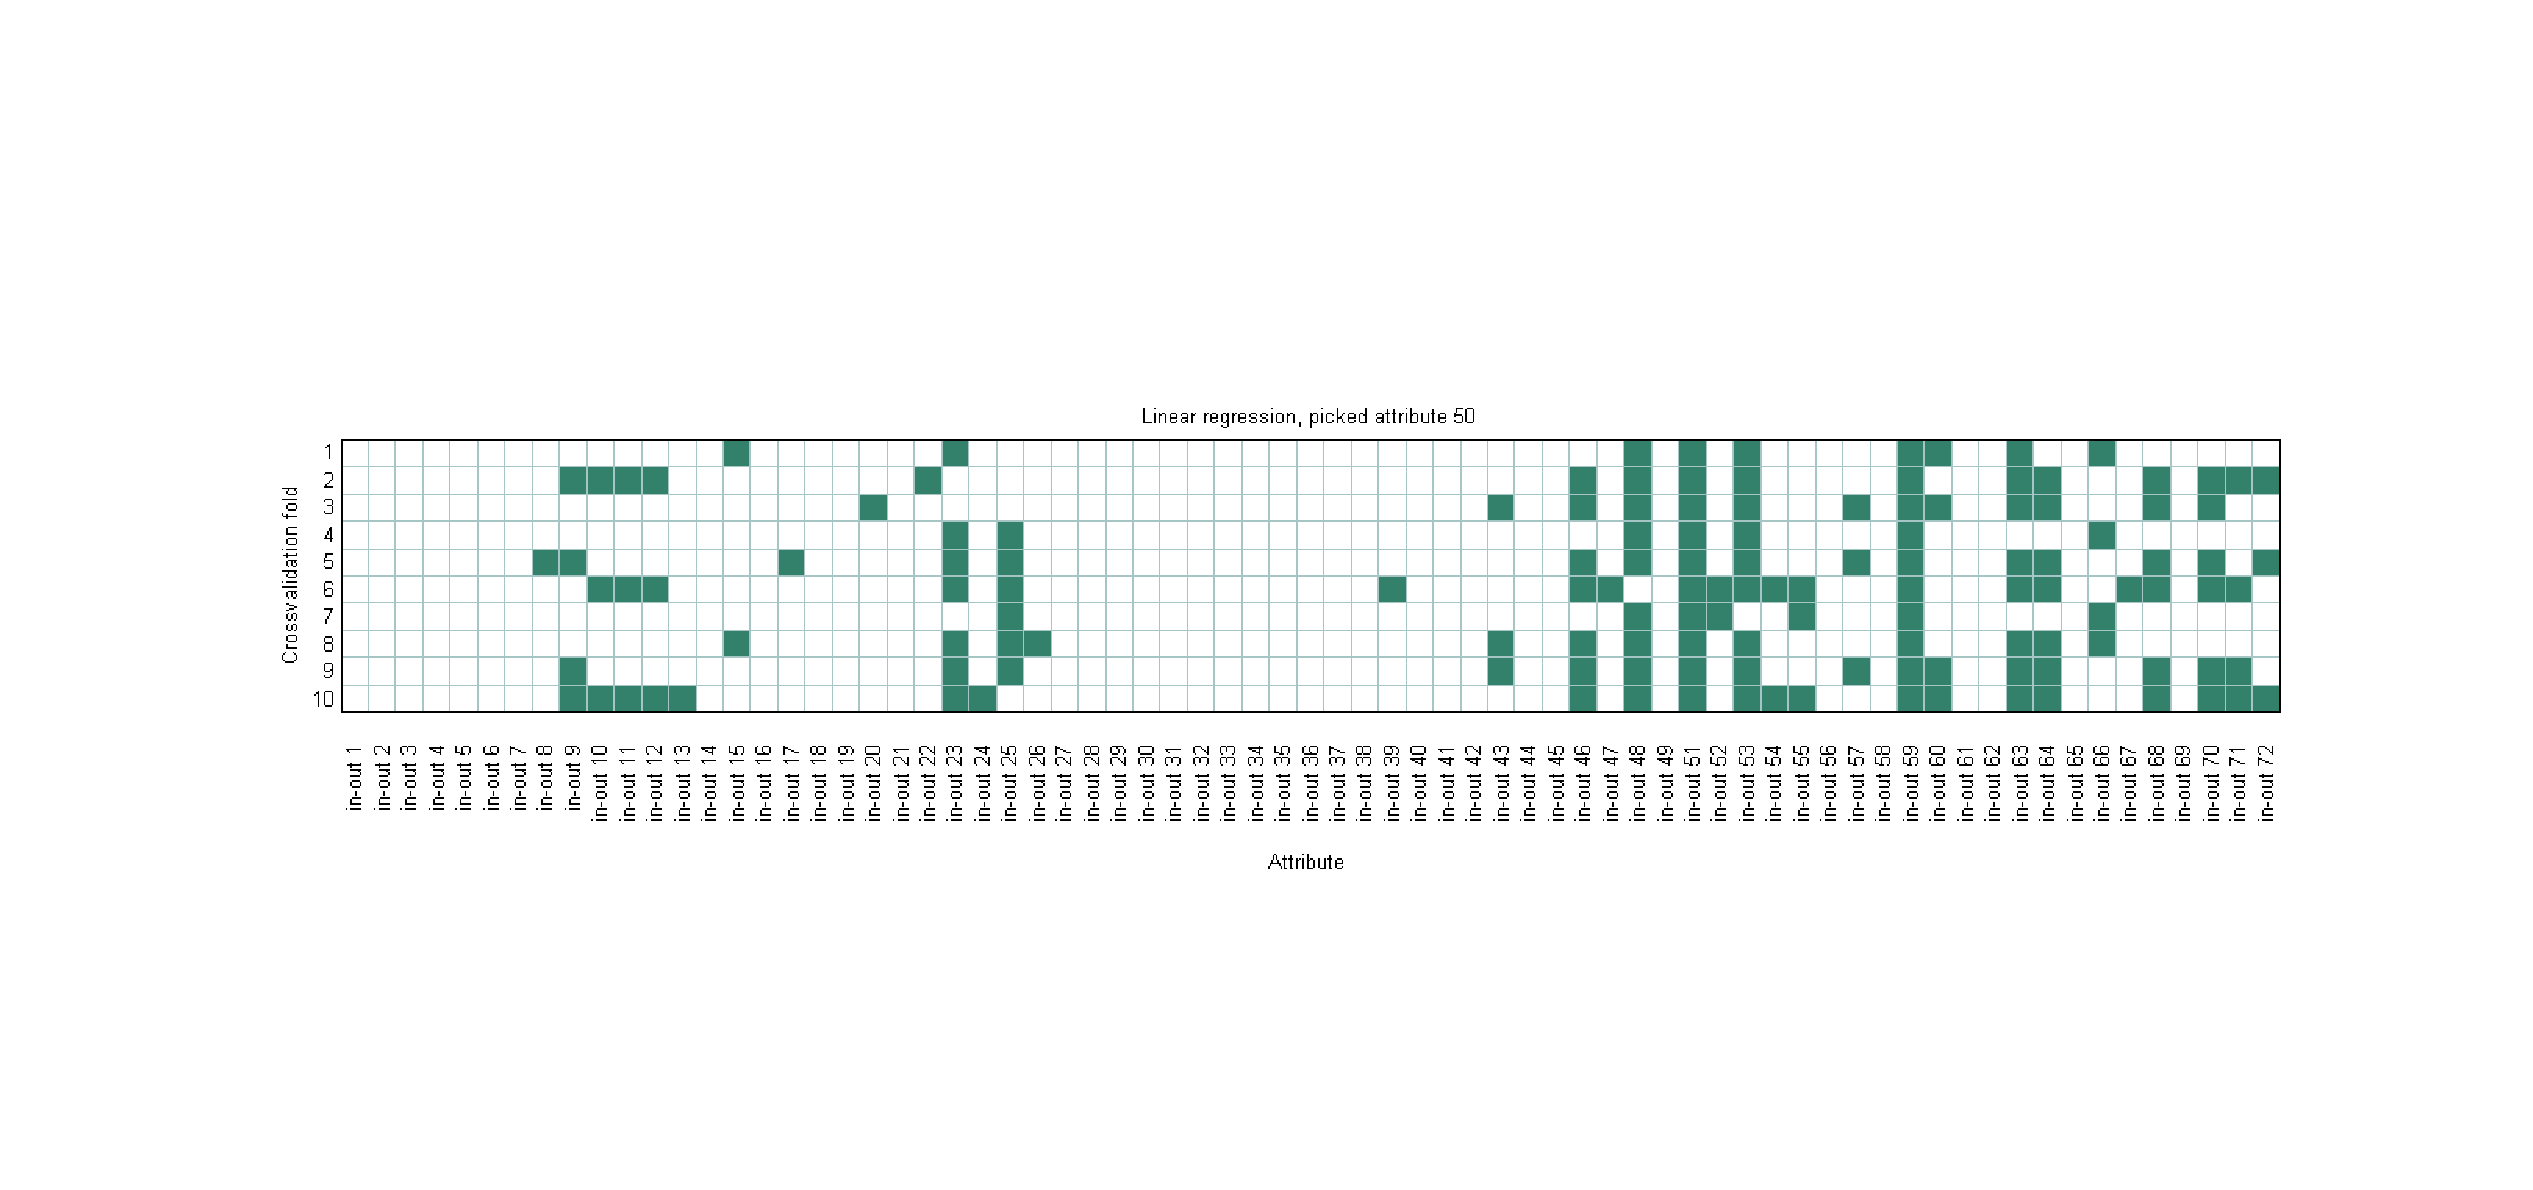
\includegraphics[width=\linewidth, trim= 50mm 50mm 50mm 60mm, clip]{code/linear_regression_attr50}
\caption{Linear regression with forward feature selection when for predicting feature \texttt{'In-out 50'}. The feature selection for each of the cross-validation is shown. Not many features are selected in order to achieve the best outcome in each cross-validation.}
\label{fig:linforward_attr50}
\end{figure}

From this we can see that it tends to be features near the extracted feature (no. 50), which makes sense since they are usually quite correlated (see previous report), when dealing within the same section. \\

The resulting squared error for this feature, both with and without the feature selection:

\begin{verbatim}
Linear regression without feature selection:
- Training error:     0.05
- Test error:         0.06
- R^2 train:         0.95
- R^2 test:         0.94
Linear regression with sequential feature selection:
- Training error:     0.06
- Test error:         0.06
- R^2 train:         0.95
- R^2 test:         0.94
\end{verbatim}

Quite decent error rate when trying to predict the feature, which means that it would be viable to predict it with this approach. It is interesting to see that it also does not seem to overfit even without feature selection and still accomplishes a decent error rate here.

\subsection*{Predicting feature 'In-out 31'}

We set the number 31 feature in the In-out section to be our feature to predict, and extract this from our feature set of the 72 features. 


Then we did forward feature selection with 5-fold cross-validation (since it was significantly slower), and the selected features from this is shown below:

\begin{figure}[H]
\centering
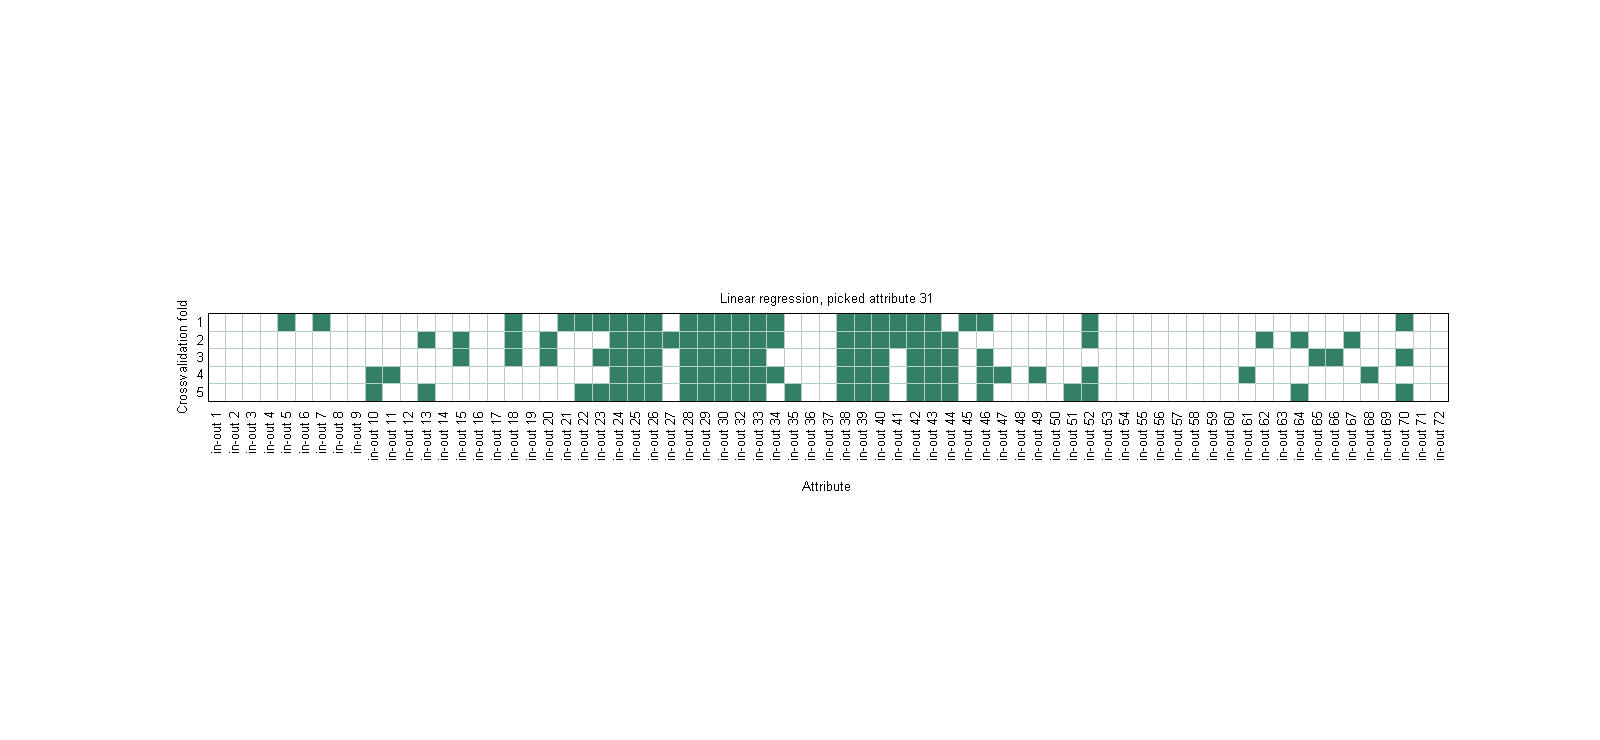
\includegraphics[width=\linewidth, trim= 50mm 50mm 50mm 70mm, clip]{code/linear_regression_attr31}
\caption{Linear regression with forward feature selection when for predicting feature \texttt{'In-out 31'}. The feature selection for each of the cross-validation is shown. More features needed when trying to predict this certain feature compared to attribute 50 from before.}
\label{fig:linforward_attr31}
\end{figure}

Again we can see that the features close to the picked one (no. 31) are often used in the feature selection. A lot more features has been selected for each cross-validation, and this explains why it was much slower at spitting out our result. \\

The resulting squared error for this feature, both with and without the feature selection:

\begin{verbatim}
Linear regression without feature selection:
- Training error:     0.54
- Test error:         0.57
- R^2 train:         0.90
- R^2 test:         0.89
Linear regression with sequential feature selection:
- Training error:     0.55
- Test error:         0.57
- R^2 train:         0.90
- R^2 test:         0.89
\end{verbatim}

This time it is much worse, and it does \emph{not} seem very viable to predict this certain feature with basic linear regression.

\subsection*{Overall}
Some features are quite possible to predict, while others are much more difficult using only linear regression. Predicting a single feature with \emph{all} of our original 272 features might be better these cases, but we are not really able to test this because of the immense computation-time for this report.

The distribution of values in the two features are quite distinct as well as seen in Figure ~\ref{attr_hist}.

\begin{figure}[H]
\centering
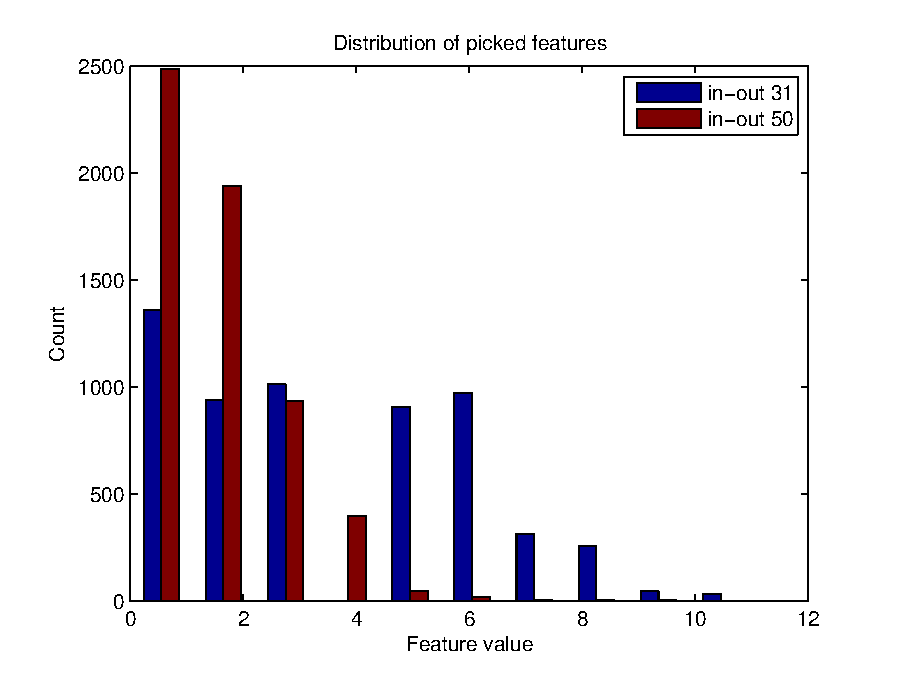
\includegraphics[width=0.6\linewidth]{code/attribute_histograms}
\caption{Distribution of values for the two extracted features. One can see that the one with low error rate is dominated by 0 and 1 entries, meaning it is easier to guess right, while the other one is more equally distributed amongst its values.}
\label{fig:attr_hist}
\end{figure}

This clearly shows that the \texttt{'In-out 31'} feature is more evenly spread, while \texttt{'In-out 50'} is mainly around 0 making it easier to predict. This is likely the reason behind the differences in error rate for these two, since \texttt{'In-out 31'} seems more erratic and/or random than the other one.

\section{New data observation}
% Explain how a new data observation is predicted according to the estimated
% model. I.e. what are the effects of the selected attributes in terms of predicting
% the data.
% (Notice, if you interpret the magnitude of the estimated coefficients this in
% general requires that each attribute be normalized prior to the analysis.).
As noted in the two examples above, the features which have something to say about the missing feature tend to be close to it. This makes sense since we deal in pixel histograms and profiles, which tend to not vary much from one feature to the ones right next to it -- it is usually a more gradual change in each way (see previous report with all features shown side-by-side for some observations).


\section{Artificial Neural Network}
% Fit an artificial neural network (ANN) model to the data.
% (You could consider only fitting the ANN to the attributes that were selected
% when you applied linear regression with forward selection).
For both our examples we fitted an ANN models to the same data. We fitted all of our ANN models with just 10 hidden units, did 5-fold cross-validation and averaged their error rates. 

\subsection*{In-out 50}
The average squared error rate for the \texttt{'In-out 50'}:

\begin{verbatim}
Error rate: 0.012
\end{verbatim}

It already had a good squared error rate using basic linear regression, but it is now $~5$ times better with ANN -- from $0.06$ to $0.012$.

\subsection*{In-out 31}
For \texttt{'In-out 31'} the resulting error rate became:

\begin{verbatim}
Error rate: 0.035
\end{verbatim}

Which greatly improves the squared error rate compared to the linear regression. From a huge error rate of $0.57$ on the test data, to only $0.035$! Making it $\frac{0.57}{0.035} \approx 16$ times better \\

A paired t-test between these two seems excessive since we can already clearly see that the ANN beats the linear regression significantly regarding the average error rates.

%\section{Performance comparison}
% Statistically evaluate if there is a significant performance difference between
% the fitted ANN and linear regression models based on the same cross-validation
% splits (i.e., use a paired t-test). Compare in addition if the performance of your
% models are better than simply predicting the output to be the average of the
% training data output.